  A tabela \ref{opnioes2iteracao} descreve o \textit{feedback} dos usuários com os pontos que faltaram na aplicação:
	
  \begin{table}[h]
  \centering
  \begin{tabular}{|m{1.5cm}||m{15cm}|}
    \hline
    \textbf{Usuário} & \textbf{Sentiu falta de:}\\
    
    \hline                               
    1 & 
      \begin{itemize}
	\item Deixar as informações na tela mais divididas.
	\item Uma opção ao usuário de registro.
      \end{itemize}\\

    \hline                               
    2 & 
      \begin{itemize}
	\item Cancelar a edição da notificação.
	\item Fazer confirmação de alterado com sucesso.
      \end{itemize}\\
    
    \hline                               
    3 & 
      \begin{itemize}
	\item Programar para aviso prévio (não no dia).
	\item A cidade ser a primeira a ser selecionada para limitação do seventos.
      \end{itemize}\\
    
    \hline                               
    4 & 
    \begin{itemize}
      \item Deixar o "Não" destacado da opção de excluir notificação.
    \end{itemize}\\
    
    \hline                               
    5 & 
    \begin{itemize}
      \item Não há sugestões.
    \end{itemize}\\
    
    \hline
  \end{tabular}
  \caption{Opniões dos usuários na 2ª iteração de avaliação.}
  \label{opnioes2iteracao}
  \end{table}
  
  
  
  Na figura \ref{resposta_asq_2iteracao} se encontram as respostas ao questionário ASQ pelos cinco usuários avaliados.

  
  
  \begin{figure}[!htb]
  \centering
  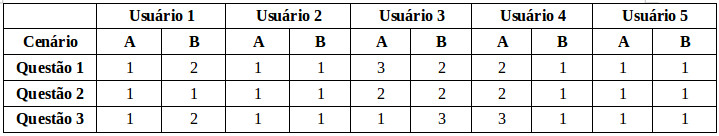
\includegraphics[scale=0.6]{figuras/nota2avaliacao.jpg}
  \caption{Resposta dos usuários ao questionário ASQ na segunda avaliação do protótipo de papel}
  \label{resposta_asq_2iteracao}
  \end{figure}